% !TEX TS-program = pdflatex
% !TEX encoding = UTF-8 Unicode

% This is a simple template for a LaTeX document using the "article" class.
% See "book", "report", "letter" for other types of document.

\documentclass[11pt]{article} % use larger type; default would be 10pt

\usepackage[utf8]{inputenc} % set input encoding (not needed with XeLaTeX)

%%% PAGE DIMENSIONS
\usepackage{geometry} % to change the page dimensions
\geometry{a4paper} % or letterpaper (US) or a5paper or....

\usepackage{graphicx} % support the \includegraphics command and options

\usepackage{amssymb}
\usepackage{amsmath}
%%% PACKAGES
\usepackage{booktabs} % for much better looking tables
\usepackage{array} % for better arrays (eg matrices) in maths
\usepackage{paralist} % very flexible & customisable lists (eg. enumerate/itemize, etc.)
\usepackage{verbatim} % adds environment for commenting out blocks of text & for better verbatim
\usepackage{subfig} % make it possible to include more than one captioned figure/table in a single float
% These packages are all incorporated in the memoir class to one degree or another...

%%% HEADERS & FOOTERS
\usepackage{fancyhdr} % This should be set AFTER setting up the page geometry
\pagestyle{fancy} % options: empty , plain , fancy
\renewcommand{\headrulewidth}{0pt} % customise the layout...
\lhead{}\chead{}\rhead{}
\lfoot{}\cfoot{\thepage}\rfoot{}

%%% SECTION TITLE APPEARANCE
\usepackage{sectsty}
\allsectionsfont{\sffamily\mdseries\upshape} % (See the fntguide.pdf for font help)
% (This matches ConTeXt defaults)

%%% ToC (table of contents) APPEARANCE
\usepackage[nottoc,notlof,notlot]{tocbibind} % Put the bibliography in the ToC
\usepackage[titles,subfigure]{tocloft} % Alter the style of the Table of Contents
\renewcommand{\cftsecfont}{\rmfamily\mdseries\upshape}
\renewcommand{\cftsecpagefont}{\rmfamily\mdseries\upshape} % No bold!
\usepackage{graphicx}
\graphicspath{ {./pings/} }

\usepackage{amsmath}
\DeclareMathOperator*{\argmax}{arg\,max}
\DeclareMathOperator*{\argmin}{arg\,min}

\newcount\colveccount
\newcommand*\colvec[1]{
        \global\colveccount#1
        \begin{pmatrix}
        \colvecnext
}
\def\colvecnext#1{
        #1
        \global\advance\colveccount-1
        \ifnum\colveccount>0
                \\
                \expandafter\colvecnext
        \else
                \end{pmatrix}
        \fi
}

%%% END Article customizations

%%% The "real" document content comes below...

\title{Macro PS6}
\author{Michael B. Nattinger\footnote{I worked on this assignment with my study group: Alex von Hafften, Andrew Smith, and Ryan Mather. I have also discussed problem(s) with Emily Case, Sarah Bass, and Danny Edgel.}}

%\date{} % Activate to display a given date or no date (if empty),
         % otherwise the current date is printed 

\begin{document}
\maketitle

\section{Question 1}
\subsection{Part 1}
When the government moves first, they make their choice by predicting the household's response to each choice, and the government will choose the optimal outcome. The government will expect that the households will take action $\xi_L \Rightarrow x_L$ if the government chooses $y_L,$ and choose $\xi_H \Rightarrow x_H$ if the government chooses $y_H$. The utilities from these outcomes are 12,24 respectively so the government will choose $y_H$, implying that the household chooses $x_H$. Thus, the Ramsey outcome is $(x_H,x_H,y_H)$.

When the government moves second, the households use backwards induction to determine the government's choice conditional on each possibility of household choice, then determine the outcome which is optimal for them. In this case, the households will assume that the government will choose $y_L$. The household will then choose $\xi_L \Rightarrow x_L$. After making this choice, the government will choose $y_L$ because $u(x_L,x_L,y_L)=12>0 = u(x_L,x_L,y_H)$. Thus, the Nash equilibrium is $(x_L,x_L,y_L).$
\subsection{Part 2}
The Ramsey outcome cannot be supported because $u(x_H,x_H,y_L) = 25>24 = u(x_H,x_H,y_H)$. Thus, for any finite number of iterations of the economy, in the final period the government will choose $y_L$ and so the households will anticipate this and choose $x_L$. In the second-to-last period, the government then has no incentive to choose $y_H$ so they will choose $y_L$ in that period, which the households will anticipate so they will choose $x_L,$ and so the government in the third-to-last period has no incentive to choose $y_H$, etc.
\subsection{Part 3}
As in the first section, the Ramsey equilibrium of the extended case will be $(x_H,x_H,y_H)$. There is still one Nash equilibria at $(x_L,x_L,y_L).$ However, now there exists a second Nash equilibria at $(x_{LL},x_{LL},y_{LL}).$ We can use this third nash equilibrium as a punishment-equilibrium to allow the Ramsey outcome to be supported. Thus, the strategy households can adopt is to choose $x_H$ in the first two periods and $x_L$ in the third period, with any deviation of the government from the equilibrium path resulting in the households choosing $x_{LL}$ for all remaining periods.

In the first period, the households will choose $x_H$. The government will then choose whether to stay on the equilibrium path or deviate. If they stay on the equilibrium path, they will receive the following utility: $24 + \beta 24 + \beta^2 12 = 55.32 $. However, if they deviate they will receive $25 + \beta 2 +\beta^2 2 = 28.42$. So, clearly in this period they will not deviate from the equilibrium path, and will choose $y_H$. In the second period the households will again choose $x_H$ and the government will consider to stay on the equilibrium path, resulting in a utility of $24+\beta 12 = 34.8$, or to deviate, resulting in a utility of $25 +\beta 2 = 26.8$. So, clearly the government will choose to stay on the equilibrium path for periods one and two, and in the third period the households choose $x_L$ and the government chooses $y_L$ as planned. 

\section{Question 2}
\subsection{Part 1}
The planner chooses labor, leisure, and government spending to maximize utility, subject to the resource constraint of the economy:
\begin{align*}
&\max_{l,g,c} \text{ln }l +\text{ln }(\alpha + c) +\text{ln }(\alpha + g)\\
&\text{s.t. } l+g+c = 1
\end{align*}
where we have imposed consistency, i.e. $l = \bar{l},c = \bar{c}$. We can use the budget constraint to write $l$ as a function of $g,c$, and substitute it into the utility function. We can thus rewrite the optimization problem as the following:
\begin{align*}
&\max_{l} \text{ln }(1-c-g) +\text{ln }(\alpha + c) +\text{ln }(\alpha + g)
\end{align*}

Taking FOCs:
\begin{align*}
\frac{\partial u}{\partial l} = 0 &\Rightarrow 1-c-g = \alpha + c \\
\frac{\partial u}{\partial l} = 0 &\Rightarrow 1-c-g = \alpha + g \Rightarrow c=g \\
&\Rightarrow 1-2c = \alpha + c \Rightarrow c = \frac{1-\alpha}{3} = g\\
&\Rightarrow l = 1 - 2\frac{1-\alpha}{3} = \frac{2\alpha +1}{3}.
\end{align*}
Thus, the planner will set $(c,l,g) = \left( \frac{1-\alpha}{3} , \frac{2\alpha +1}{3}, \frac{1-\alpha}{3}  \right)$.

\subsection{Part 2}
In the Ramsey equilibrium, the government moves first. The government will predict how the households will react to a given tax rate and will set tax to optimize the utility given the expected household reaction. 

Given a set tax level $\tau,$ the household will maximize utility subject to their budget constraint:
\begin{align*}
&\max_{l,c} \text{ln }l +\text{ln }(\alpha + c) +\text{ln }(\alpha + g)\\
&\text{s.t. } c \leq (1-\tau)(1-l)
\end{align*}

It is clear that the budget constraint will hold with equality. We can use the budget constraint to rewrite the optimization problem:
\begin{align*}
&\max_{l} \text{ln }l +\text{ln }(\alpha + (1-\tau)(1-l)) +\text{ln }(\alpha + g)
\end{align*}

Taking FOCs:
\begin{align*}
\frac{\partial u}{\partial l} = 0 &\Rightarrow (1/l) - \frac{1-\tau}{\alpha + (1-\tau)(1-l)} = 0 \Rightarrow l = \frac{\alpha}{1-\tau} +1 - l \\
&\Rightarrow l = \frac{\alpha}{2(1-\tau)} + \frac{1}{2}\\
&\Rightarrow c = (1-\tau)\left(1/2 -\frac{\alpha}{2(1-\tau)}  \right) = (1-\tau - \alpha)/2.
\end{align*}

The government will take these quantities for granted and choose $\tau$ to optimize utility:
\begin{align*}
&\max_{\tau} \text{ln }\left(\frac{\alpha}{2(1-\tau)} + \frac{1}{2}\right) +\text{ln }\left(\alpha + (1-\tau - \alpha)/2\right) +\text{ln }\left(\alpha + \tau\left(1- \frac{\alpha}{2(1-\tau)} - \frac{1}{2} \right)\right)\\
\Rightarrow &\max_{\tau}  \text{ln }\left(\frac{\alpha}{2(1-\tau)} + \frac{1}{2}\right) +\text{ln }\left( (1-\tau + \alpha)/2\right) +\text{ln }\left(\alpha + \tau\left(\frac{1}{2}- \frac{\alpha}{2(1-\tau)} \right)\right)\\
\Rightarrow &\max_{\tau}  \text{ln } (\alpha +1 - \tau) - \text{ln } (2(1-\tau)) + \text{ln }(1-\tau+\alpha) - \text{ln }2 \\&+ \text{ln }(\alpha 2(1-\tau) + \tau (1-\tau - \alpha)) - \text{ln }(2(1-\tau))\\
\Rightarrow &\max_{\tau}  \text{ln } (\alpha +1 - \tau) - \text{ln } (1-\tau) + \text{ln }(1-\tau+\alpha) - 3\text{ln }2 \\&+ \text{ln }(\alpha 2(1-\tau) + \tau (1-\tau - \alpha)) - \text{ln }(1-\tau)\\
\end{align*}
where we have substituted our expressions for government spending, as given, and simplified. Taking FOCs with respect to $\tau$,

\begin{align*}
\frac{\partial u}{\partial \tau} = 0 &\Rightarrow -(\alpha +1-\tau)^{-1} + (1-\tau)^{-1} - (1-\tau+\alpha)^{-1} \\&+ (\alpha 2(1-\tau) + \tau (1-\tau - \alpha))^{-1}(-2\alpha + (1-\tau-\alpha)-\tau) +(1-\tau)^{-1} =0\\
&\Rightarrow -2(1-\tau+\alpha)^{-1} + 2(1-\tau)^{-1} +\frac{-3\alpha + 1 - 2\tau}{2\alpha(1-\tau) + \tau(1-\tau-\alpha)} = 0.
\end{align*}
This has no analytical solution, and we will solve for later parts using a numerical solution on a grid of $\alpha$ values in Matlab (as recommended by Katya).

Values for $c,l,\tau,g$ for the Ramsey equilibrium for a given level of $\alpha$ are plotted below.

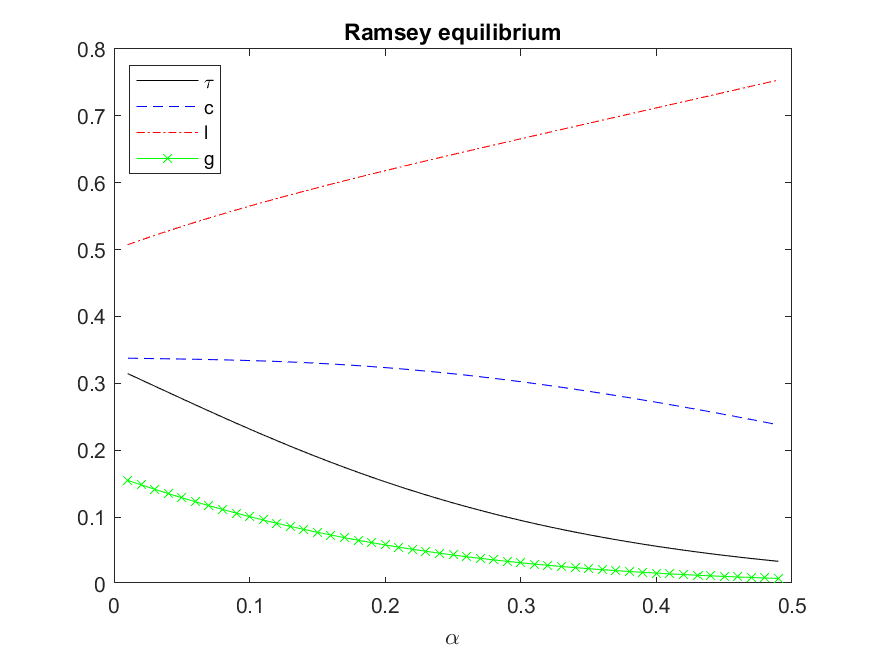
\includegraphics{ramsey}

%\begin{align*}
%\frac{\partial u}{\partial \tau} = 0 &\Rightarrow \left(\frac{\alpha}{2(1-\tau)} + \frac{1}{2}\right)^{-1}\left(\frac{-\alpha}{2(1-\tau)^2} \right) + \left( (1-\tau + \alpha)/2\right) ^{-1}\left( -\frac{1}{2} \right) \\&+ \left(\alpha + \tau\left(\frac{1}{2}- \frac{\alpha}{2(1-\tau)} \right)\right)^{-1}\left(\left(\frac{1}{2}- \frac{\alpha}{2(1-\tau)} \right) +\tau\left( \frac{\alpha}{2(1-\tau)^2}\right) \right) = 0 \\
%&\Rightarrow \left(\frac{2(1-\tau)}{\alpha+(1-\tau)}\right)\left(\frac{-\alpha}{2(1-\tau)^2} \right) - \frac{1}{1-\tau+\alpha} \\&+ \left(\frac{2(1-\tau)}{(1-\tau)(2\alpha+\tau) - \tau\alpha}\right)\left(\frac{(1-\tau)^2 - \alpha + 2\alpha \tau}{2(1-\tau)^2} \right) = 0 \\
%&\Rightarrow \left(\frac{-\alpha}{\alpha(1-\tau)+(1-\tau)^2}\right) - \frac{1}{1-\tau+\alpha} \\&+ \left(\frac{1}{(1-\tau)(2\alpha+\tau) - \tau\alpha}\right)\left(\frac{(1-\tau)^2 - \alpha + 2\alpha \tau}{(1-\tau)} \right) = 0 \\
%\end{align*}

%\begin{align*}
%\frac{\partial u}{\partial \tau} = 0 &\Rightarrow  \frac{3a+2\tau -1}{3a\tau - 2a + \tau^2 - \tau} + \frac{2}{-a+\tau -1} - \frac{2}{\tau-1} = 0\\%\frac{1}{2}\left( \frac{\frac{\alpha}{1-\tau} +1}{2}\right)^{-1}\frac{\alpha}{(1-\tau)^2} + \frac{1}{2(\alpha +1 - \tau)}+\frac{(1-\tau)^2 - a}{(\tau - 1)(a(3\tau - 2) +(\tau -1)\tau)}% \left(\alpha + \frac{\tau}{2} - \frac{\tau\alpha}{2(1-\tau)} \right)^{-1}(\frac{1}{2})= 0 \\
%&\Rightarrow 2\alpha +2\tau = \frac{\alpha}{\tau\alpha +\tau^2}
%\end{align*}

%We can set up and solve our lagrangian as follows:
%
%\begin{align*}
%\mathcal{L} &=  \text{ln }\left( \frac{\frac{\alpha}{1-\tau} +1}{2}\right) +\text{ln }\left((\alpha +1-\tau )/2\right) +\text{ln }\left(\alpha + g\right) + \lambda \left(g-\tau\left(1- \frac{\frac{\alpha}{1-\tau} +1}{2}\right)\right)\\
%\frac{\partial \mathcal{L}}{\partial g} = 0 &\Rightarrow \frac{1}{\alpha+g} +\lambda = 0\\
%\frac{\partial \mathcal{L}}{\partial \tau} = 0&\Rightarrow \left( \frac{\frac{\alpha}{1-\tau} +1}{2}\right)^{-1}
%%\Rightarrow &\max_{\tau} \text{ln }\left( \frac{\frac{\alpha}{1-\tau} +1}{2}\right) +\text{ln }\left((\alpha +1 - \tau )/2\right) +  \text{ln }\left(\alpha + \frac{\tau}{2} - \frac{\tau\alpha}{2(1-\tau)} \right)
%\end{align*}

\subsection{Part 3}
The households will act first. They will anticipate the government's taxation strategy, and choose their labor supply to maximize their own utility given that strategy. So, the households figure out $\tau$ by setting:
\begin{align*}
\tau = \argmax_{\tau} f(\tau) = \argmax_{\tau} \text{ln }l +\text{ln }(\alpha + (1-\tau) (1-l)) +\text{ln }(\alpha + \tau(1-l)) 
\end{align*}
Taking first order conditions,
\begin{align*}
\frac{\partial f}{\partial \tau} = 0 &\Rightarrow \frac{-(1-l)}{(\alpha + (1-\tau) (1-l))} + \frac{(1-l)}{\alpha + \tau(1-l)} = 0\\
&\Rightarrow (1-l)\alpha + \tau (1-l)^2 = \alpha(1-l) + (1-\tau)(1-l)^2 \\
&\Rightarrow 2\tau = 1 \Rightarrow \tau = \frac{1}{2},
\end{align*}
or $l=1$. We will work through the case where $\tau=\frac{1}{2}$ first and then check the corner solution $l=1$ at the end.

The household solves the following optimization problem:
\begin{align*}
\max_{l} f(l) &= \max_{l} \text{ln }l +\text{ln }(\alpha + (1/2) (1-l)) +\text{ln }(\alpha + g) \\
\frac{\partial f}{\partial l} = 0 &\Rightarrow l^{-1} -\frac{1/2}{\alpha + (1/2)(1-l)} = 0\\
&\Rightarrow l = 2\alpha + 1 - l \\
&\Rightarrow l = \alpha + \frac{1}{2}\\
&\Rightarrow c = \frac{1}{4} - \frac{1}{2}\alpha \\
&\Rightarrow g = \frac{1}{4} - \frac{1}{2}\alpha
\end{align*}

\subsection{Part 4}
The households work less in the Nash equilibrium than in the planner's solution because the households try to avoid the distortionary taxes.  Consumption and government spending are still equilized in both equilibria owing to the shape of the household's utility function.

As we calculated the Ramsey equilibrium numerically, we will compare the solutions graphically.

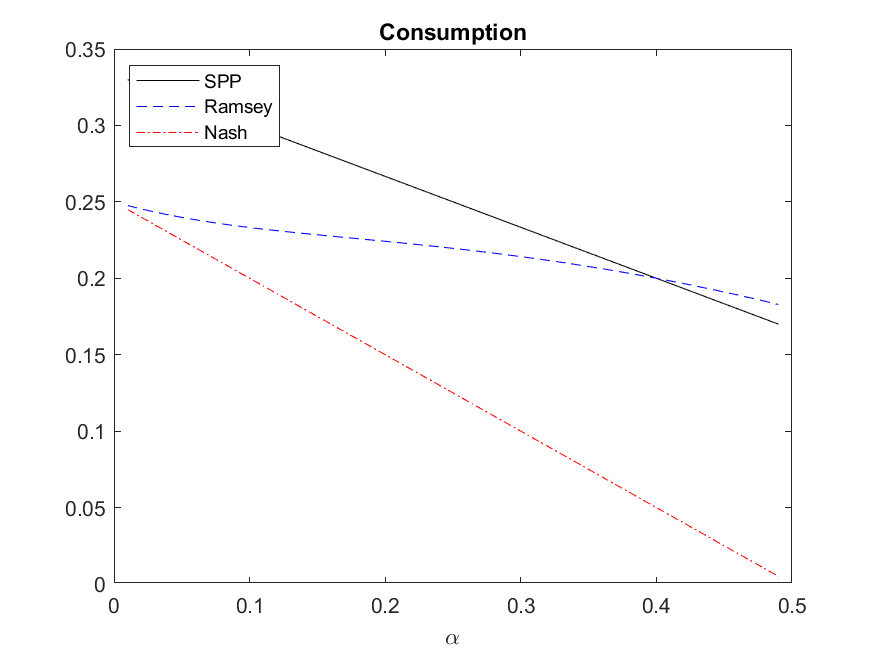
\includegraphics{cons}
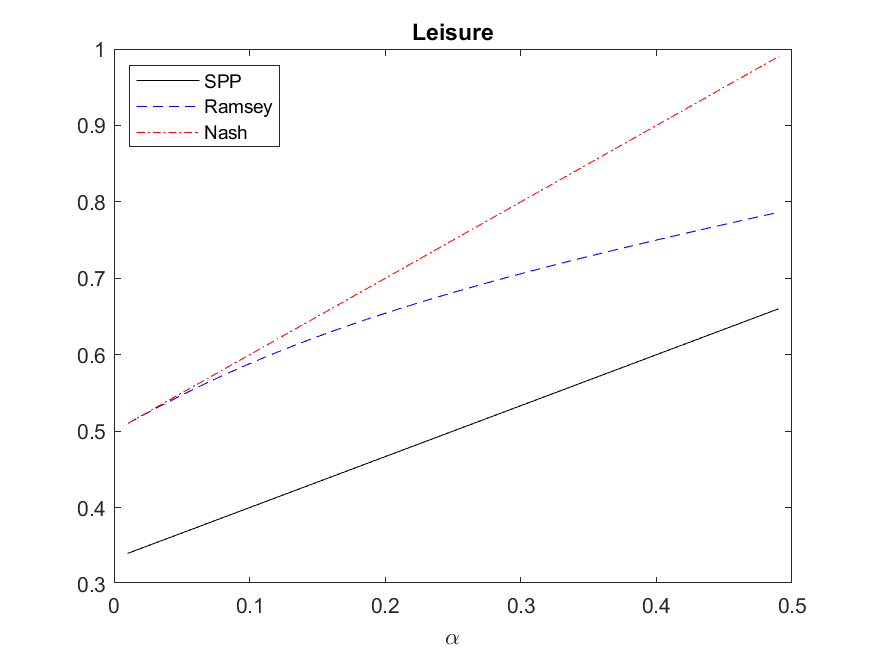
\includegraphics{leisure}
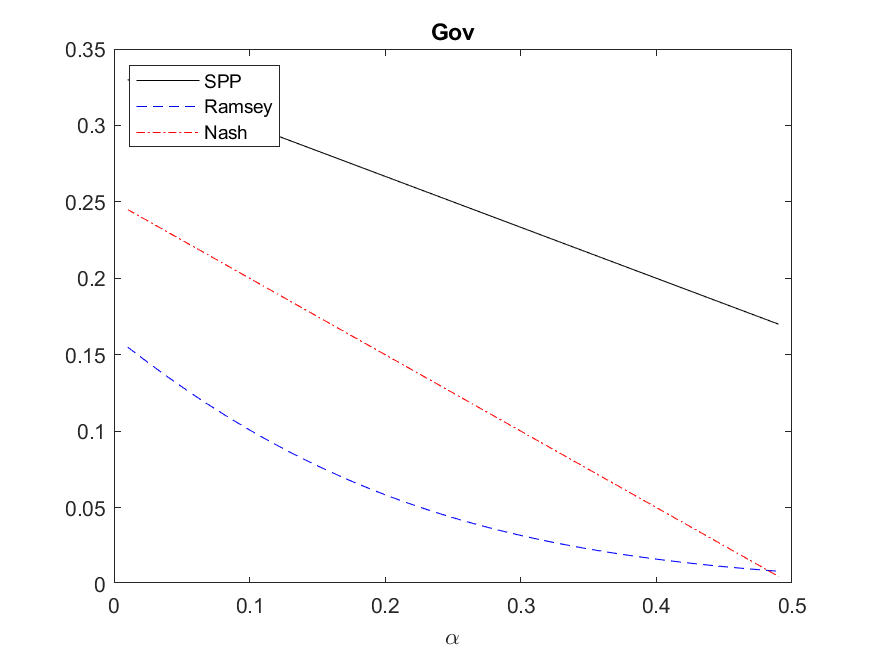
\includegraphics{gov}
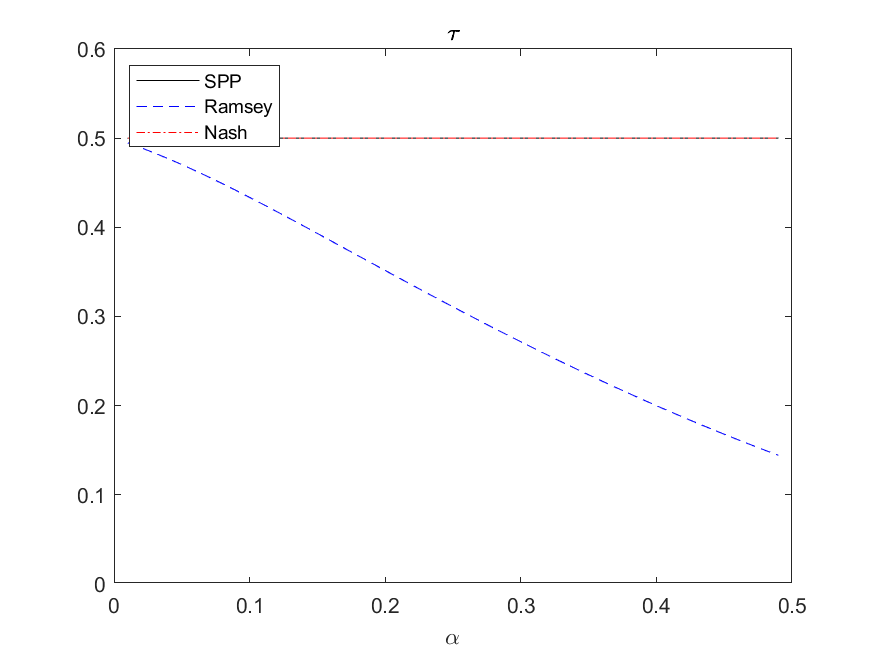
\includegraphics{tau}
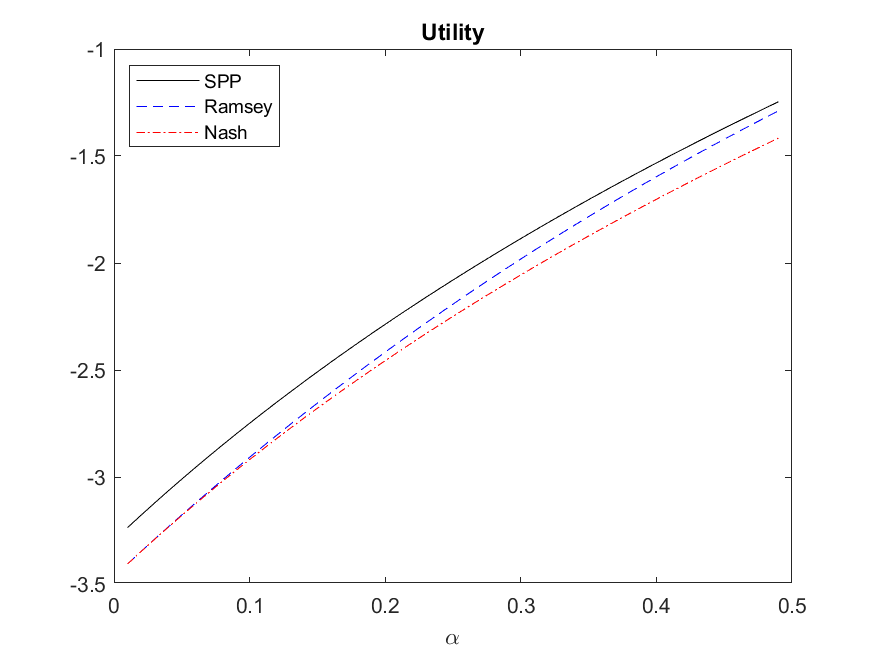
\includegraphics{util}
As expected, the SPP equilibrium dominates both the Ramsey equilibrium and the Nash equilibrium. Also, the Ramsey equilibrium dominates the Nash equilibrium for all periods.

In the Ramsey equilibrium, the government always selects a lower value of $\tau$ than they would like to implement in either the SP or Nash equilibrium. This is so that the consumers have a greater incentive to work. As the value of $\alpha$ increases, the amount of $\tau$ the government imposes drops as the higher $\alpha$ value makes up for the reduced government spending.

\subsection{Part 5}

We can support the Ramsey equilibrium if the following inequality holds:
\begin{align*}
u(l_R|\tau = \tau_R) + \sum_{i=1}^{\infty} \beta^i u(l_R|\tau=\tau_R)&>u(l_R|\tau = \tau_N) + \sum_{i=1}^{\infty} \beta^i u(l_N|\tau=\tau_N)\\
\Rightarrow \frac{1}{1-\beta}u(l_R|\tau = \tau_R)  &> u(l_R|\tau = \tau_N) + \frac{\beta}{1-\beta}u(l_N|\tau=\tau_N)
\end{align*}
where the subscript R denotes the Ramsey equilibrium, and the subscript N denotes the Nash equilibrium. We can solve for the minimum such value of $\beta$ for a givven level of $\alpha$ in Matlab.

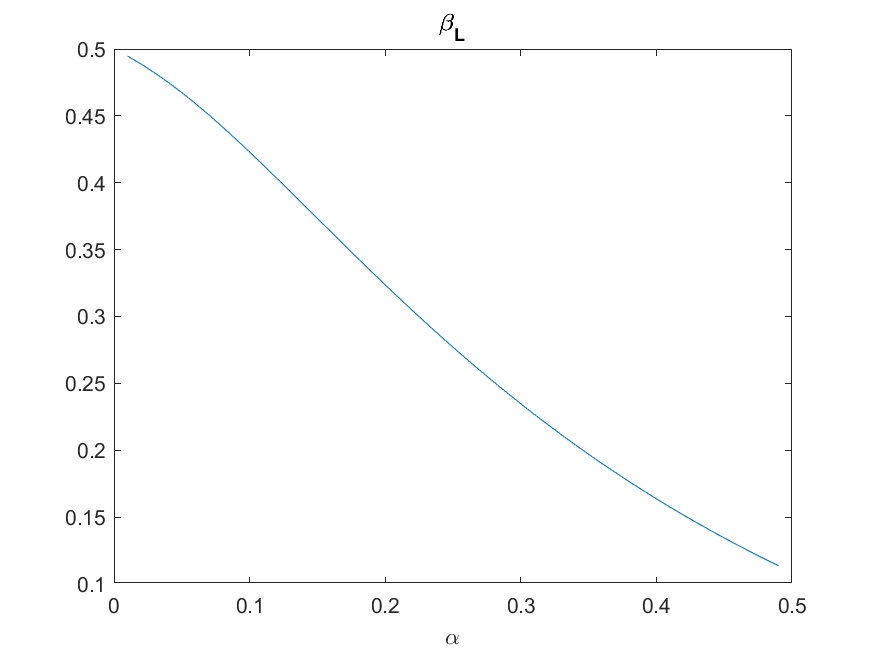
\includegraphics{beta}

The above figure plots the minimum $\beta$ necessary for the Ramsey equilibrium to be supported at a given value of $\alpha$.
\end{document}
